\documentclass[a4paper]{article}

\usepackage[swedish]{babel}
\usepackage[T1]{fontenc}
\usepackage[utf8]{inputenc}
\usepackage{graphicx}
\usepackage{float}

\newcommand\namn{Larmsystem}

\restylefloat{table}

\begin{document}


\thispagestyle{empty}

\begin{center}
    \parskip=14pt
    \vspace*{3\parskip}

    {\LARGE Projektplan DAT290}

    {\large \namn, grupp 11

    Titus Blosse, Viktor Frideen, Nazif Kadiroglu, Markus Moen, Lukas Schiavone, Fredrik Österström

    \today}

    \rule{7cm}{0.4pt}\\
\end{center}
\newpage

\thispagestyle{empty}

\tableofcontents
\newpage


\pagenumbering{arabic}

\section{Syfte}
Inbrott är ett vanligt problem i Sverige. År 2019 anmäldes 75.250 inbrottstölder. En minskning med 14\% från året innan \cite{brastold}. Vanliga sätt att förhindra inbrott är grannsamverkan, certifierade lås mot inbrott och hemlarm. Larmsystem minskar risken för ett inbrott och möjliggör ytterligare minskning både i Sverige och i resten av världen.

\section{Mål}

Produkten ska erbjuda ett flertal larmkomponenter som kan anslutas till en larmcentral och konfigureras för att passa kundens specifika situation. Systemet ska vara dokumenterat och fackmannamässigt utfört med förutsättningar för expansion.

Grunden i systemet kommer vara en centralenhet till vilken användaren kan ansluta periferienheter. Huvudsakligen kommer två periferienheter att utvecklas, ett dörrlarm och ett rörelselarm.

I mån av tid kommer extra uppgifter utföras. Uppgift 1 och uppgift 4 kommer prioriteras. Om ytterligare tid finns kommer även uppgift 2 och 3 att implementeras.

%Har förtydligat att vi kommer försöka med extra uppgifter. Kanske ska ändra om vilka extra uppgifter vi vill göra dock. /Titus

%Ett testläge för systemet, möjlighet att konfigurera rörelselarmet, och ett inbyggt skydd mot så kallade ``replay attacker'' kommer prioriteras.

\section{Bakgrund}

Beståndsdelarna i larmsystemet är en centralenhet och periferienheter. Komponenterna skapar tillsammans möjligheten att till exempel, larma på/av, koppla samman enheter eller inställning av befintliga enheter. Koppling sker via instruktioner som kan skickas både manuellt eller automatiskt via en av komponenterna.

\subsection{Begrepp}

\begin{description}
    \item[CAN:] Controller Area Network
    \item[MD407:] Mikrodator av typen MD407
\end{description}


\subsection{Tekniska förutsättningar}

Hårdvaran för att driva larmsystemet är utvecklad och dokumenterad. Tre mikro-datorer av typen MD407 driver periferienheterna och centralenheten. För kommunikation mellan datorerna används CAN (Controller Area Network)-protokollet, för detta finns ett kodexempel. Periferienheterna använder sensorer för att upptäcka störningar och initiera ett alarm som skickas till centralenheten. Till varje periferienhet kopplas en sensor av typen dörr-, vibrations- eller avståndssensor. Detta möjliggör tre över två olika kombinationer av sensorer med periferienheterna.

\section{Systemöversikt}

\begin{figure}[H]
    \centering
    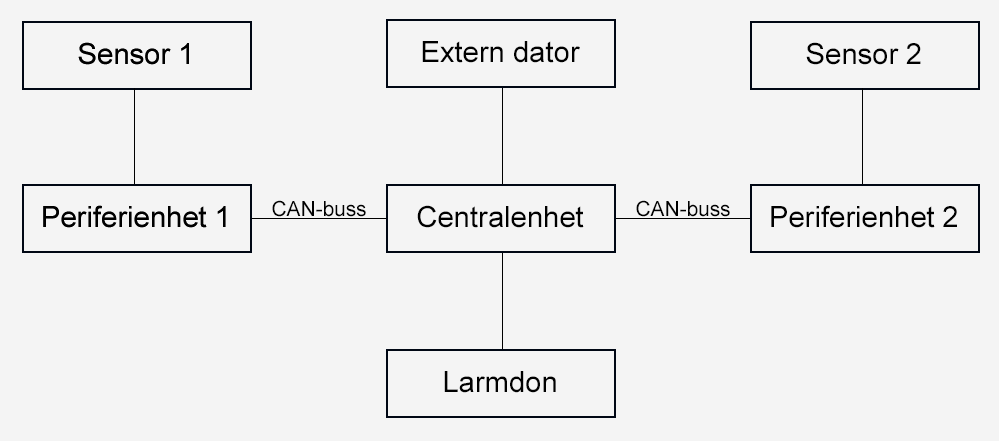
\includegraphics[width=\textwidth]{blockschema.png}
    \caption{Preliminärt blocksschema över larmsystemet}
\end{figure}

Centralenheten kommunicerar med periferienheterna genom en CAN-buss. Periferienheterna undersöker ändringar hos deras sensorer och vid funnen ändring rapporteras detta till centralenheten för alarm. Inrapporteringen sker via ett meddelande på bussen som skapar ett avbrott hos centralenheten och aktiverar larmdonet.

Centralenheten måste kunna identifiera vilken periferienhet som skickat meddelandet och förstå varför det skickades. Identifikationen sker via kommunikation med en extern dator för att ge användaren en tydlig bild om var alarmet uppstod.

\section{Resursplan}

E-mailadresser och ansvarsområden finns angivna i följade lista. Ansvar syftar på att den ansvarige ska se till att arbetet blir gjort, men inte att den ansvarige är skyldig att göra allt.

\subsection{Gruppmedlemmar och ansvarsområden}

\begin{description}
    \item[Titus Blosse, administrativt dokumentansvarig:] Ansvarar för att mötesprotokoll förs och att de olika rapporterna som ska skrivas under projektets gång såväl påbörjas som skickas in i tid.

    E-mail: titus.blosse@gmail.com

    \item[Viktor Frideen, planeringsansvarig:] Ansvarar för att informera gruppen om hur arbete med projektet och dess delmål fortgår och även för att uppmärksamma gruppen om de hamnar efter planeringen.

    E-mail: viktor.frideen@outlook.com

    \item[Nazif Kadiroglu, teknik dokumentansvarig:] Ansvarar för att all kod i projektet är dokumenterad och att dokumentationen följer förutbestämd struktur.

    E-mail: nazif.kadiroglu1@gmail.com

    \item[Markus Moen, testansvarig:] Ansvarar för att hårdvara och mjukvara testas och att testerna dokumenteras.

    E-mail: markus.offersten@gmail.com

    \item[Lukas Schiavone, kodansvarig:] Ansvarar för att gruppen följer den förutbestämda kodstandarden.

    E-mail: luksch1121@gmail.com

    \item[Fredrik Österström, gruppledare och resursansvarig:] Ansvarar för kommunikation med kursens lärare och gruppmöten, hårdvarans tillgänglighet och att de verktyg gruppen har valt för kommunikation och versionhantering används.

    E-mail: fredrik.osterstrom@hotmail.com
\end{description}

\subsection{Arbetsfördelning}

\begin{description}
    \item[Kommuniationsprotokoll] Ansvarande gruppmedlemmar: Markus Moen och Titus Blosse. Kommuniationsprotokoll innefattar kommunikation mellan de olika enheterna.
     
    \item[Perifirienheter] Ansvarande gruppmedlemmar: Nazif Kadiroglu och Viktor Frideen. Perifirienheter innefattar utveckling av dörr- och rörelselarmen.
     
    \item[Centralenhet] Ansvarande gruppmedlemmar: Lukas Schiavone och Fredrik Österström. Centralenhet innefattar mottagning och bearbetning av data från perifirienheter, såväl som utveckling av användargränssnitt.
\end{description}

Arbetsfördelningen ovan kan variera. De olika arbetsgrupperna kommer samarbeta med varandra flytandes under projektet då de olika delarna överlappar. Detta innebär att arbetsgrupperna asnvarar för deras respektive delar, men även att gruppmedlemmar flexibelt kan hjälpa varandra. 

\subsection{Hård- och mjukvara}

Hårdvaran för detta projekt finns tillgänglig i rum 4209 i EDIT-huset på Chalmers campus Johanneberg. Rummet och hårdvaran bokas via Doodle. Länkar till bokningssystemet finns på kurshemsidan. Hårdvaran som finns tillgänglig är:

\begin{itemize}
    \item 3x MD407 kort
    \item 1x Avståndsmätare (ultraljud), HC-SR04
    \item 1x Vibrationssensor, "Flying-Fish" SW-18010P
    \item 1x Keypad
    \item 1x 7-segmentsdisplay
    \item 2x 4-polig RJ-11 kabel (används för CAN-bussen)
    \item 1x RJ-11 förgrening
    \item 2x Tiopolig flatkabel
    \item 3x USB-kabel
    \item 1x Kopplingsplatta
\end{itemize}

Programspråket C kommer användas för att skriva mjukvaran. Den IDE (Integrated Design Environment) som kommer användas är CodeLite då gruppmedlemmarna redan har erfarenthet med denna IDE. CodeLite kan även simulera MD407-korten med hjälp av programvaran SimServer. GitHub används för versionhantering.

En del av arbetet kan ske på distans, men för att utföra test på hårdvaran krävs det att gruppmedlemmar är på plats i Chalmers.

\section{Milstolpar}


\begin{table}[H]
    \centering
        \begin{tabular}{ |c|c|c| }\hline
            Nr & Beskrivning & Datum \\\hline \hline
            1 & Projektplan klar & 11/09-20 \\\hline
            2 & Dörrlarm klart & 18/09-20 \\\hline
            3 & Kommunikationsprotokoll & 25/09-20 \\\hline
            4 & Rörelselarm klart & 25/09-20 \\\hline
            5 & Centralenhet delvis avklarad & 02/10-20 \\\hline
            6 & Första utkast slutrapport & 02/10-20 \\\hline
            7 & Centralenhet och periferienheter sammankopplade & 09/10-20 \\\hline
            8 & Opposition avklarad & 09/10-20 \\\hline
            9 & Andra utkast slutrapport & 16/10-20 \\\hline
            10 & Slutrapport avklarad & 30/10-20 \\\hline
        \end{tabular}
        \caption{Milstolpar för projektet}
        \label{table:milstolpar}
\end{table}

För att underlätta projektet har arbetet delats in i nio olika milstolpar. Milstolparna är placerade fredagen innan slutdatumet då det lämnar utrymme för mer arbete om så behövs.

Programmeringsarbetet har delats in i fyra delar. Först utvecklas dörrlarmet och sedan rörelselarmet. Därefter utvecklas centralenheten och slutligen skall periferienheterna och centralenheten sammankopplas.

\section{Aktiviteter}

Gruppmedlemmarna förväntas spendera 200h vardera med ett totalt antal mantimmar motsvarande 1200h. Tiden som varje medlem i gruppen förväntas lägga ner innefattar all tid som spenderas på projektet.

\begin{table}[H]
    \begin{center}
        \begin{tabular}{ |c|c|c| }\hline
            Nr & Beskrivning & Tidsåtgång \\\hline\hline
            1 & Föreläsningar (8 st på 2h, ett skrivseminarium på 3h, 6 personer) & 114h \\\hline
            2 & Dokumentationsläsning & 50h \\\hline
            3 & Framtagning av LaTeX-mallar & 18h \\\hline
            4 & Projektmöten (2h/vecka, 9 veckor, 6 personer) & 108h \\\hline
            5 & Skrivande av protokoll, kallelser etc & 20h \\\hline
            6 & Arbeta med projektplan & 120h \\\hline
            7 & Rapportutkast & 120h \\\hline
            8 & Renskrivande av Rapportutkast 1 & 15h \\\hline
            9 & Rapportutkast 2 & 80h\\\hline
            10 & Renskrivning av rapportutkast 2 & 10h \\\hline
            11 & Oppositionsrapport & 40h\\\hline
            12 & Slutföring av projektrapport & 110h\\\hline
            13 & Programmering av periferienhet, dörr & 40h \\\hline
            14 & Programmering av periferienhet, rörelse & 40h \\\hline
            15 & Programmering av centralenhet & 60h \\\hline
            16 & Tester och testrapport & 100h\\\hline
            17 & Granskning av kod & 60h \\\hline
            18 & Teknisk dokumentation & 60h \\\hline
            19 & Förbered/genomför demonstration & 35h \\\hline
        \end{tabular}
        \caption{Aktivitetslista för projektet}
        \label{table:aktivitetslista}
    \end{center}
\end{table}

Projektet har delats upp i aktiviteter för att gruppen ska ha koll på vad som ska genomföras. Noterbart är att aktiviteterna har givits en uppskattad tidsåtgång i tabell \ref{table:aktivitetslista}. Tabell \ref{table:aktivitetslista} visar att gruppen sammanlagt kommer lägga cirka 1200 timmar på projektet. Dessa timmar sorteras in på 19 aktiviteter och fyra kategorier.

\begin{description}
    \item[Aktivitet 1-3] berör inläsningen och förarbetet gruppen kommer göra under projektet. (182h)

    \item[Aktivitet 4-5] berör det administrativa arbetet. (128h)

    \item[Aktivitet 6-12] berör den skriftliga delen av projektet. (495h)

    \item[Aktivitet 13-19] berör den praktiska delen av projektet. Detta innefattar programmering, test och demonstrationer. (395h)

\end{description}


\section{Tidsplan}
\begin{figure}[H]
    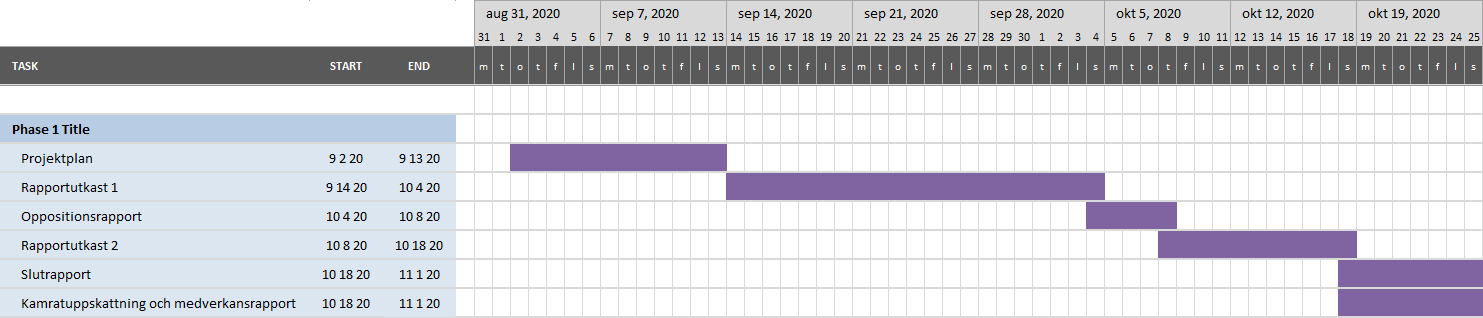
\includegraphics[width=\textwidth]{Gantt-Schema1.png}
    \caption{Gantt-schema}
    \label{figure:gantt}
\end{figure}

Aktiviteter och tidsåtgång presenteras i Gantt-schemat ovan. Andra aktiviteter som inte visas i figur \ref{figure:gantt} sker kontinuerligt under projektets gång. Dessa inkluderar föreläsningar, möten, tester etc.
\begin{description}
\item [Första två veckorna] innefattar introduktion till projektet och skrivning av projektplan.

\item [När projektplan är färdigställt] börjar gruppen arbeta med den praktiska delen av projektet. Under cirka 2-4 veckors tid förväntas larmsystemet och rapportutkast 1 vara färdigt.

\item [Sista veckorna av projektet] förväntas gruppen arbeta med oppositionsrapport, rapportutkast 2 och slutrapport. Utöver detta skall varje gruppmedlem skriva en kamratuppskattning.
\end{description}

\newpage

\section{Mötesplan}

Mötestillfällen där alla gruppmedlemmar inklusive mentor medverkar.

\begin{table}[H]
    \begin{center}
        \begin{tabular}{ |c|c|c| }\hline
            Datum & tid & Lokal \\\hline\hline
            02/09-20 & 13:00-15:00 & ED4209 \\\hline
            09/09-20 & 15:00-17:00 & Zoom \\\hline
            16/09-20 & 13:00-15:00 & Zoom \\\hline
            23/09-20 & 13:00-15:00 & Zoom \\\hline
            30/09-20 & 13:00-15:00 & Zoom \\\hline
            07/10-20 & 13:00-15:00 & Zoom \\\hline
            14/10-20 & 13:00-15:00 & Zoom \\\hline
            21/10-20 & 13:00-15:00 & Zoom \\\hline
            28/10-20 & 13:00-15:00 & Zoom \\\hline
        \end{tabular}
        \caption{Tabell över mötestillfällen}
        \label{table:motesplan}
    \end{center}
\end{table}

\section{Kommunikationsplan}

\begin{table}[H]
    \centering
    \begin{tabular}{ |c|c|c|c| }\hline
     Vad & När & Till & Hur \\\hline
     Dagsordning LV1 & 02/09-20 & Alla & Anslag i Canvas \\\hline
     Mötesprotokoll LV1 & 02/09-20 & Alla & Anslag i Canvas \\\hline
     Dagsordning LV2 & 09/09-20 & Alla & Anslag i Canvas \\\hline
     Mötesprotokoll LV2 & 10/09-20 & Alla & Anslag i Canvas \\\hline
     Projektplan & 09/13-20 & Lärarteam & Inlämning i Canvas\\\hline
     Dagsordning LV3 & 16/09-20 & Alla & Anslag i Canvas \\\hline
     Mötesprotokoll LV3 & 17/09-20 & Alla & Anslag i Canvas \\\hline
     Dagsordning LV4 & 23/09-20 & Alla & Anslag i Canvas \\\hline
     Mötesprotokoll LV4 & 24/09-20 & Alla & Anslag i Canvas \\\hline
     Dagsordning LV5 & 30/09-20 & Alla & Anslag i Canvas \\\hline
     Mötesprotokoll LV5 & 01/10-20 & Alla & Anslag i Canvas \\\hline
     Projektrapport utkast 1 & 04/10-20 & Lärarteam & Inlämning i Canvas \\\hline
     Dagsordning LV6 & 07/10-20 & Alla & Anslag i Canvas \\\hline
     Mötesprotokoll LV6 & 08/10-20 & Alla & Anslag i Canvas \\\hline
     Dagsordning LV7 & 14/10-20 & Alla & Anslag i Canvas \\\hline
     Mötesprotokoll LV7 & 15/10-20 & Alla & Anslag i Canvas \\\hline
     Projektrapport utkast 2 & 18/10-20 & Läratteam & Inlämning i Canvas \\\hline
     Dagsordning LV8 & 21/10-20 & Alla & Anslag i Canvas \\\hline
     Mötesprotokoll LV8 & 22/10-20 & Alla & Anslag i Canvas \\\hline
     Dagsordning LV9 & 28/10-20 & Alla & Anslag i Canvas \\\hline
     Mötesprotokoll LV9 & 29/10-20 & Alla & Anslag i Canvas \\\hline
     Projektrapport & 03/11-20 & Lärarteam & Inlämning i Canvas \\\hline
    \end{tabular}
    \caption{Kommunikationsplan för projektet}
    \label{table:kommunikationsplan}
\end{table}
Ansvaret för den skriftliga kommunikationen har främst delats upp mellan gruppledare och dokumentansvarige. Däremot kommer gruppen gemensamt fram till datum och tid för mötestillfällen. Utöver detta kommer gruppen även ha mailkontakt med handledare.

För intern kommunikation används tjänsterna Discord och Messenger. Gruppmöten med handledare kommer i första hand att ske igenom Zoom.

\section{Kvalitetsplan}

För att verifiera att systemet och dess delsystem fungerar behöver tester utföras. Tester av mjukvaran kan i viss mån göras i simulator, men innan den kan markeras som klar måste den testas i hårdvaran. Vid test av de olika komponenterna skall följande mall fyllas i:

\begin{description}
\item[Komponent] Den del av systemet som ska testas.

\item[Testsyfte] Vilken funktionalitet som testas.

\item[Utförande] Hur testet ska utföras och vilka specifika fall som testas.

\item[Resultat] Resultatet av testet.

\item[Analys] Vad testresultatet innebär; om komponenten fungerar som planerat, behöver testas ytterligare eller om vidare utveckling krävs.
\end{description}

\bibliographystyle{IEEEtran}

\bibliography{referenser.bib}

\end{document}
